\section{Questão 01}

A primeira questão da prova considera a utilização de um sinal de eletrocardiografia (ECG) disponibilizado pelo Goldenberg no \textit{site} Goldenberg \cite{Goldberger2000}; a partirdo qua lse  extraiu uma janela de um minuto, de dois canais. Porém, para a execução do processamento, optou-se por utilizar o primeiro canal do sinal, denominado de MLII.

O sinal de ECG obtido pelo arquivo \textit{.mat} foi importado via codificação em \textit{Python}. Informações adicionais acerca do sinal como taxa de amostragem, duração da amostra, variável onde o sinal se localiza, tamanho do vetor, nome do canal, ganho aplicado ao sinal, nível de quantização e unidade de medida foram obtidas através do arquivo \textit{118e00m.info},. As informações de ganho de 200 e do \textit{offset} de 1024 podem ser utilizadas para a conversão desses sinais para os níveis de tensões obtidos na aquisição dos sinais. Porém, optou-se por utilizar nessa prova os sinais no formato como foi obtido.

Um sinal de ECG é composto por repetições de um sinal de um mesmo formado. Variações de período do ciclo e de segmentos podem ocorrer em função de diversos fatores externos e internos ao corpo. 

Devido a isso, apesar do sinal trabalhado ter a duração de 1 minuto, as representações gráficas para a questão 01 foram feitas utilizando um janelamento de 10 segundos para que se pudese observar melhor a influência de cada etapa de processamento realizada no sinal, de forma que ciclos do sinal de ECG estejam claramente visíveis. 

Além disso, os gráficos no domínio do tempo para a questão 01 utilizam a unidade de medida bruta obtida após todo o processamento de conversão analógico digital. Assim, os valores informados não se encontram em mV.
\subsection{Item a}
Inicialmente, obteve um janelamento do sinal em função do tempo em segundos.

\begin{figure}[!htb]
    \centering
    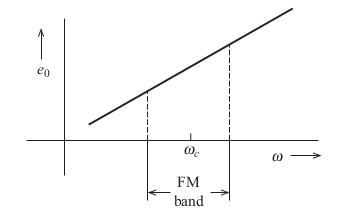
\includegraphics[width=\linewidth]{Imagens/fig01.png}
    \caption{janelamento de 10 segundos do sinal original de ECG}
    \label{fig:graph_01}
\end{figure}

Na Figura \ref{fig:graph_01}, pode-se visualizar com clareza ciclos característicos de um sinal de ECG.

\subsection{Item b}
Ao sinal visto na Figura \ref{fig:graph_01}, acrescentou-se um ruído branco gaussiano com relação sinal-ruído (SNR) de 12 decibeis (dB).

\begin{figure}[!htb]
    \centering
    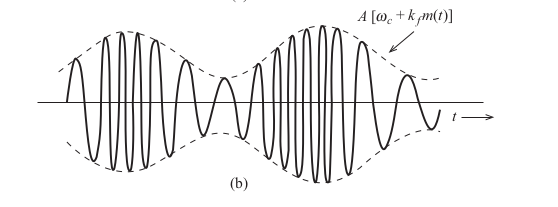
\includegraphics[width=\linewidth]{Imagens/fig02.png}
    \caption{ruído branco gaussiano adicionado ao sinal original de ECG}
    \label{fig:graph_02}
\end{figure}

Pode-se verificar na Figura \ref{fig:graph_02} que o ruído adicionado ocasinou uma grande diferença no sinal,

\subsection{Item c}
A um sinal ruidoso, pode-se utilizar um filtro que realiza a média entre amostras vizinhas. Assim, neste item, utilizou-se uma média de duas amostras. O resultado pode ser visto na Figura \ref{fig:graph_03}.

\begin{figure}[!htb]
    \centering
    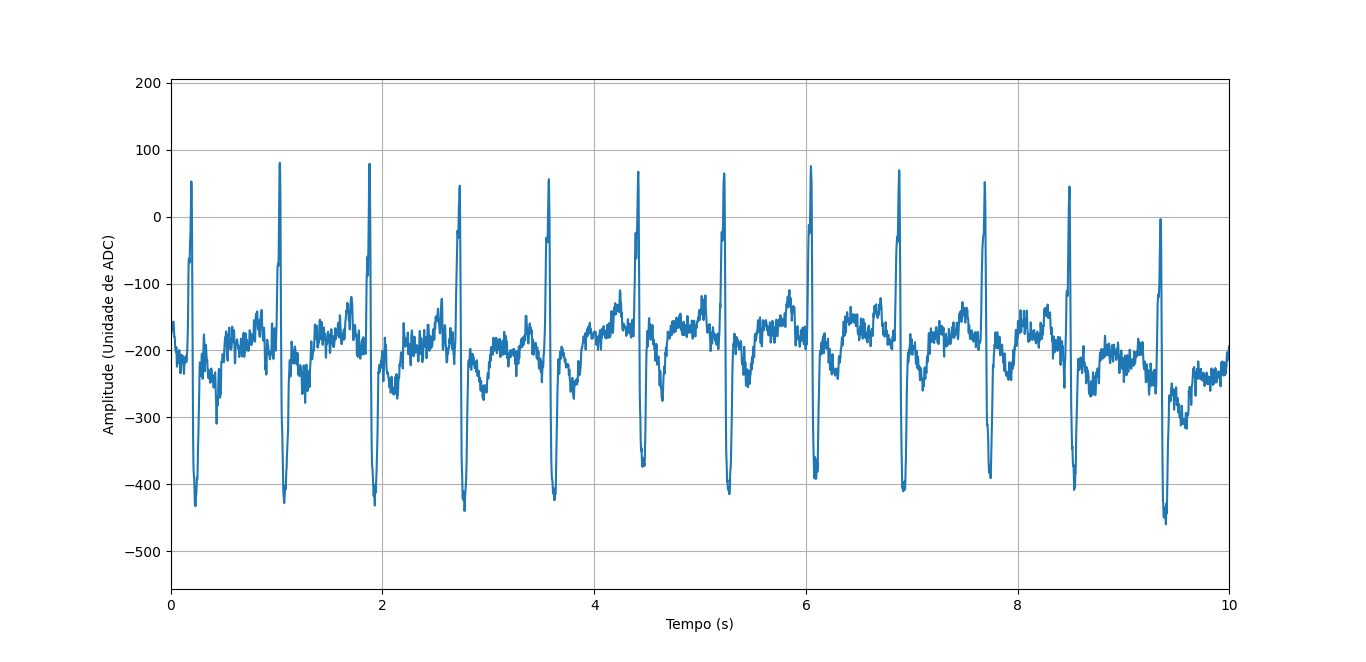
\includegraphics[width=\linewidth]{Imagens/fig03.png}
    \caption{sinal filtrado por média móvel de duas amostras}
    \label{fig:graph_03}
\end{figure}

Na Figura \ref{fig:graph_03}, observa-se uma melhora do sinal obtido. Isso acontece devido à utilização do filtro de médias. Isso acontece pois a tendência dos sinais adjacentes visa minimizar o efeito dos ruídos. 

\subsection{Item d}

Como o sinal foi amostrado a uma taxa de amostragem adequada conforme os requisitos de \textit{Nyquist}, até certo ponto, pode-se aumentar a quantidade de amostras utilizadas na média para minimizar os efeitos da presença de ruídos. Assim, aumentou-se a quantidade de amostras para 5. 

\begin{figure}[!htb]
    \centering
    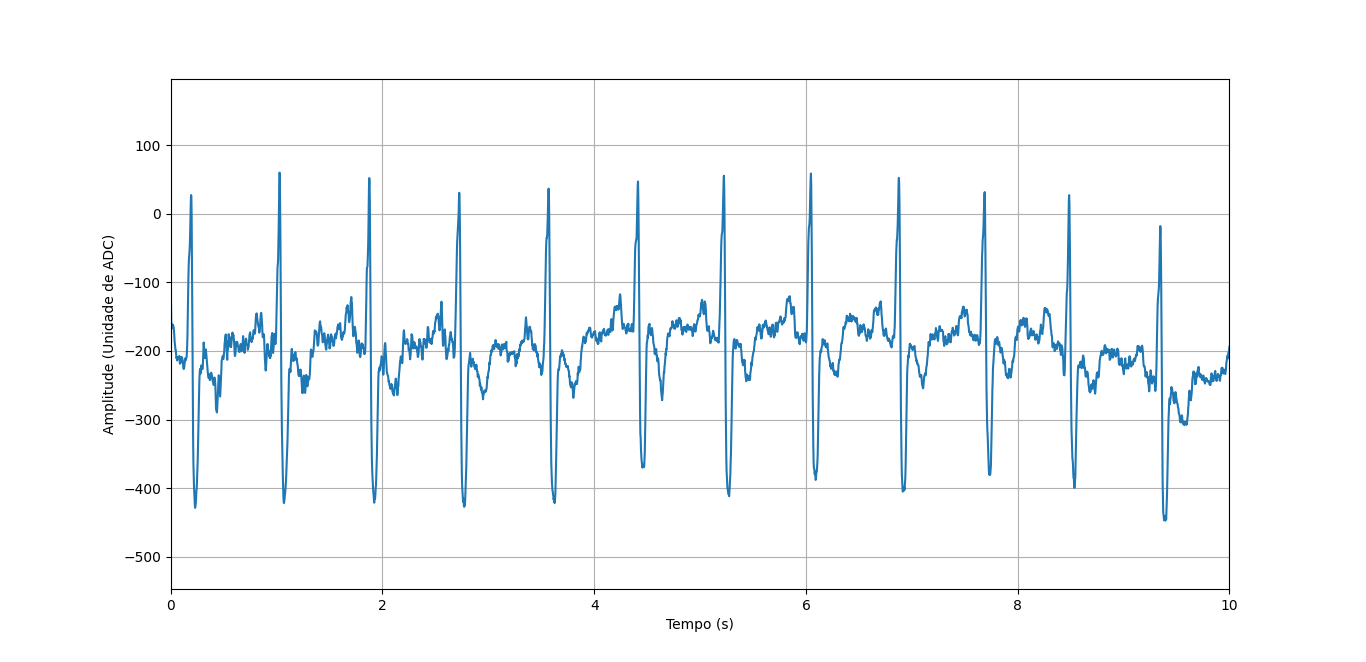
\includegraphics[width=\linewidth]{Imagens/fig04.png}
    \caption{sinal filtrado por média móvel de cinco amostras}
    \label{fig:graph_04}
\end{figure}

Na Figura \ref{fig:graph_04}, observa-se uma melhora do sinal obtido devido ao aumento de amostras utilizadas no cálculo da média.

\subsection{Item e}

Portanto, neste caso, o aumento de amostras utilizadas no cálculo de média causou uma melhora na minimazação do efeito do ruído. Porém, deve-se ficar atento à utilização desse método pois dependendo da quantidade de amostras utilizadas, os sinais podem se tornar uniformes demais. Além disso, deve-se levar em conta qual o tipo de ruído que está presente no sinal para que se elenque uma técnica adequada de filtragem.

\subsection{Item f}
Para que se aprofunde na análise do efeito da aplicação de uma filtragem de média móvel em um sinal, outra ferramenta a ser utilizada é a Transformada Discreta de Fourier de Tempo Discreto, que possibilita a representaçaõ do sinal no domínio da frequência. Representações como magnitude e fase em função de frequências pode ser uma verificação eficiente para a validação da utilização desse tipo de filtro.

Dessa forma, obteve-se as representações em magnitude e fase para os dois casos de filtragem obtidos acima.

A Figura \ref{fig:graph_05} representa a magnitude do sinal da Figura \ref{fig:graph_03}, ou seja, do sinal filtrado por média móvel de duas amostras. 

\begin{figure}[!htb]
    \centering
    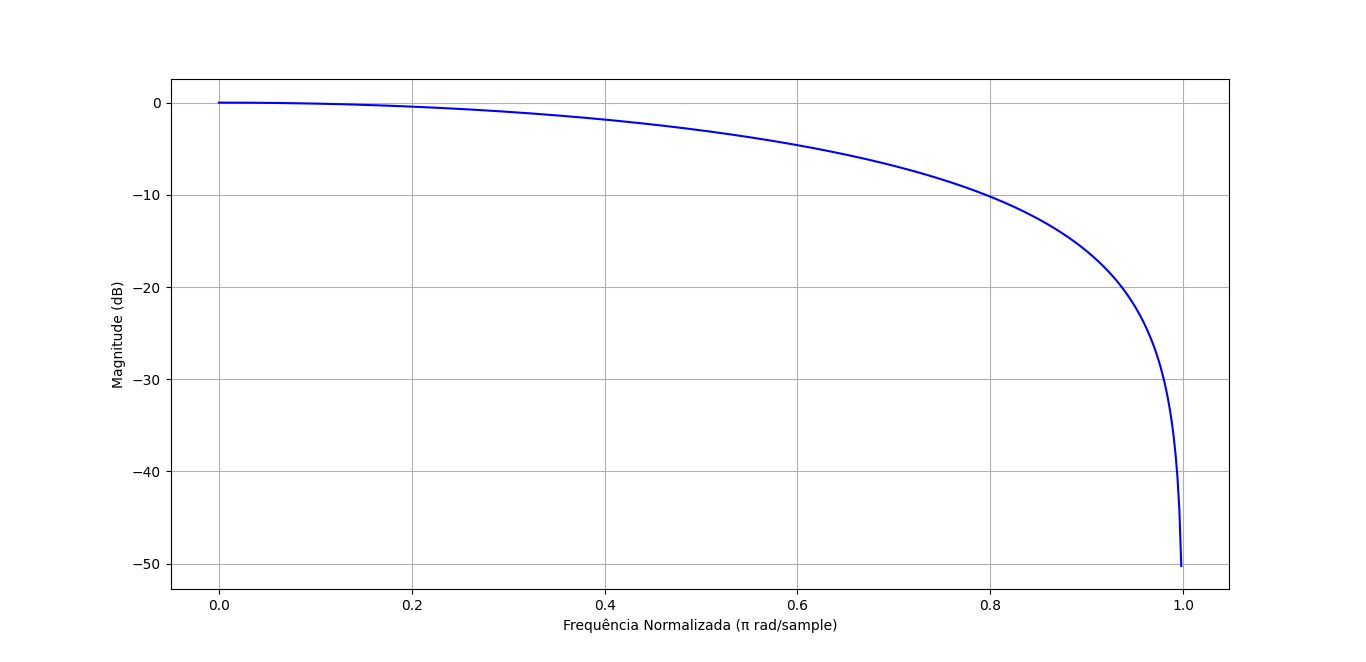
\includegraphics[width=\linewidth]{Imagens/fig05.png}
    \caption{sinal filtrado por média móvel de cinco amostras}
    \label{fig:graph_05}
\end{figure}

Ao analisar a Figura \ref{fig:graph_05}, percebe-se que as frequências próximas à frequência máxima foram bastante atenuadas.

\begin{figure}[!htb]
    \centering
    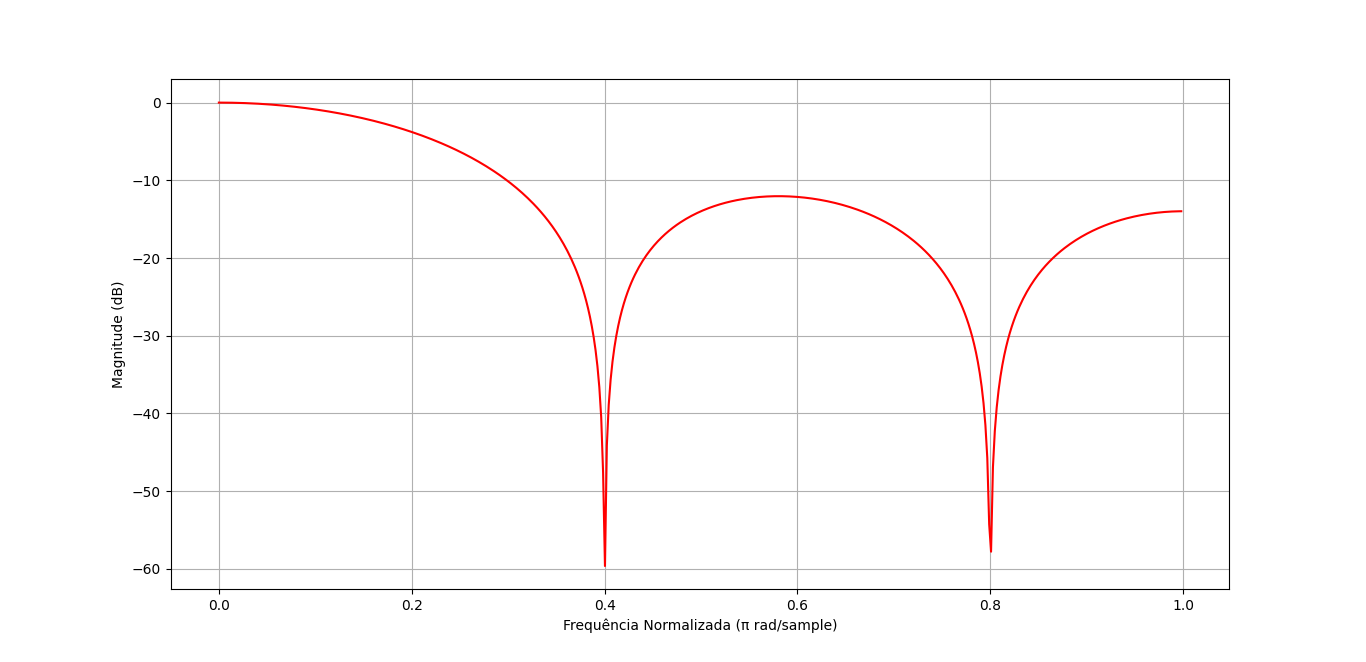
\includegraphics[width=\linewidth]{Imagens/fig06.png}
    \caption{sinal filtrado por média móvel de cinco amostras}
    \label{fig:graph_06}
\end{figure}

Já a representação da fase na Figura \ref{fig:graph_06} permite observar que houve uma distorção na fase em duas frequências. 

Ao analisar a Figura \ref{fig:graph_07}, observa-se que o filtro de média móvel de cinco amostras realizou uma atenuação da banda do sinal como um todo, gerando uma resposta linear. 

\begin{figure}[!htb]
    \centering
    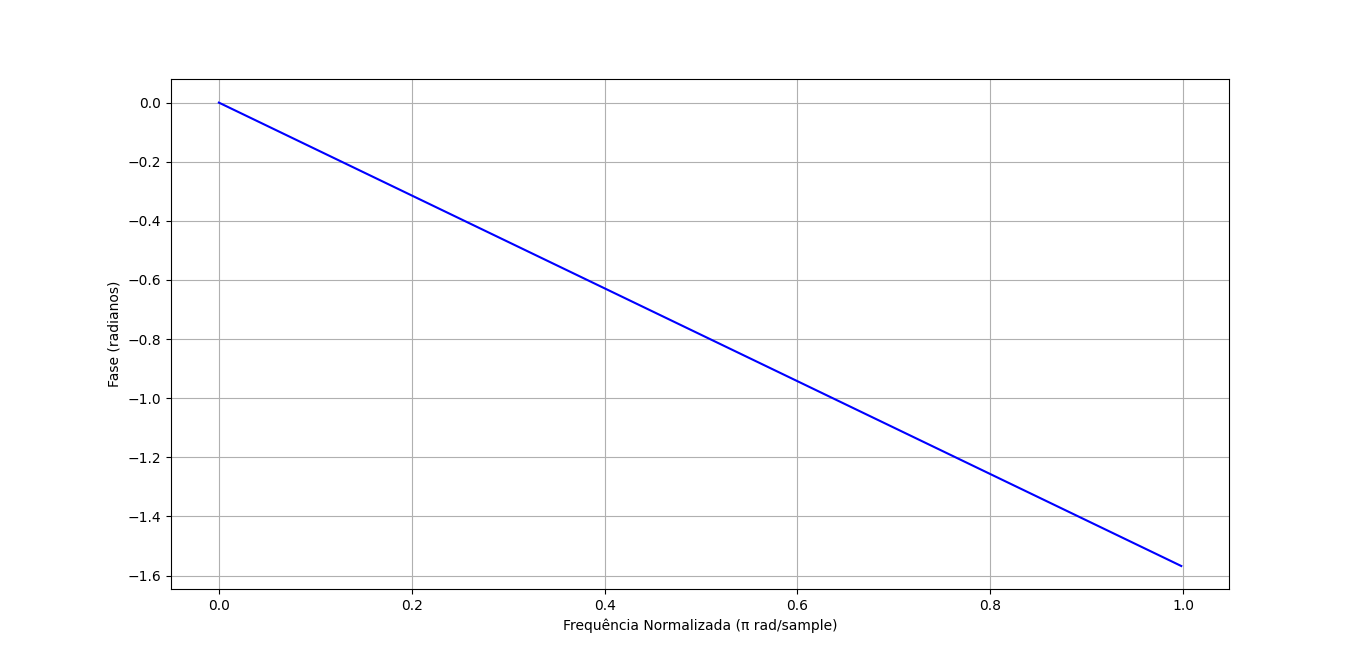
\includegraphics[width=\linewidth]{Imagens/fig07.png}
    \caption{sinal filtrado por média móvel de cinco amostras}
    \label{fig:graph_07}
\end{figure}

Em relação à defasagem do sinal, a filtragem de média móvel de cinco amostras introduziu uma resposta similar a um sinal dente de serra. Esse tipo de comportamento é obtido quando se aumenta a quantidade de amostras utilizadas em um filtro de média móvel.

\begin{figure}[!htb]
    \centering
    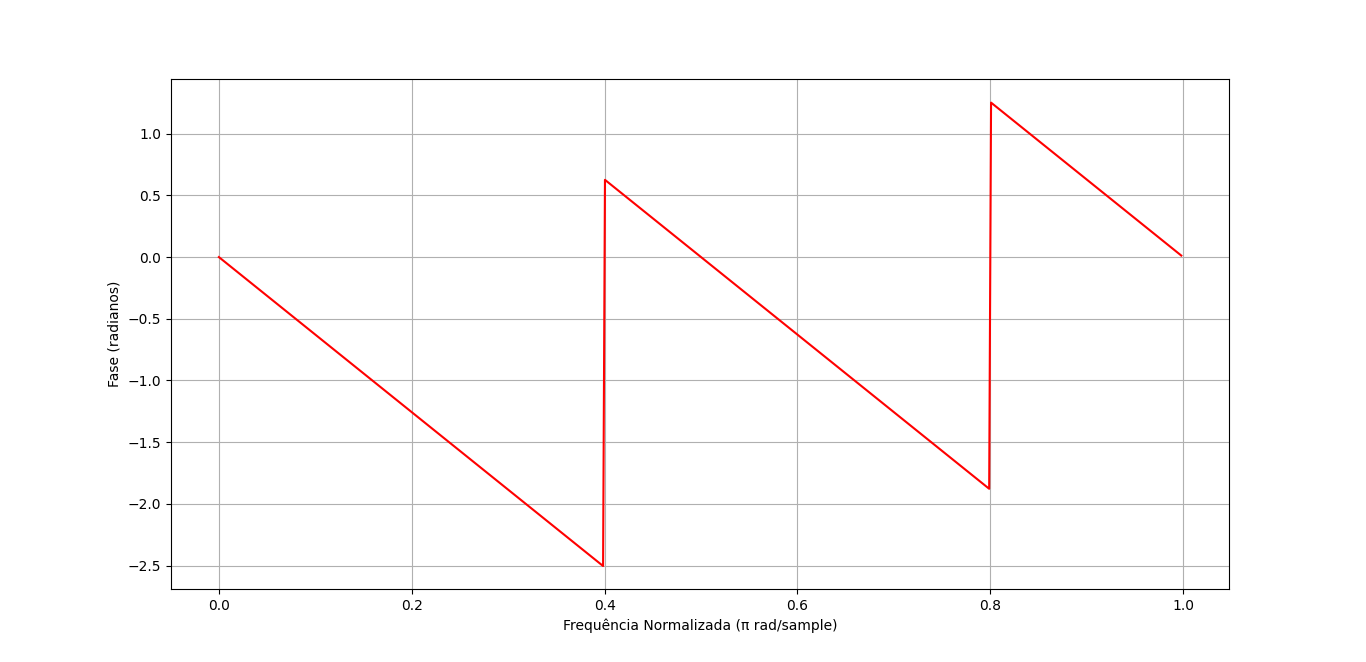
\includegraphics[width=\linewidth]{Imagens/fig08.png}
    \caption{sinal filtrado por média móvel de cinco amostras}
    \label{fig:graph_08}
\end{figure}
